\documentclass[english]{mlutalk}
% \documentclass[english,handout]{mlutalk}

\title{Grimjack at Touché 2022}
\subtitle{Axiomatic Re-ranking and Query Reformulation}
\author{Jan Heinrich Reimer \and Johannes Huck \and Alexander Bondarenko}
\institute{Martin Luther University Halle-Wittenberg\\\url{https://webis.de}}
\date{September~8, 2022}
\titlegraphic{
\includegraphics[width=3cm]{figures/mlu-halle}}

\addbibresource{../paper/literature.bib}

\usepackage{tikz}
\usetikzlibrary{positioning}
\usepackage{listings}
\usepackage{xspace}
\usepackage{biblatex}
\usepackage{tabularx}
\usepackage{booktabs}
\usepackage{graphicx}
\usepackage{tikz}
\usepackage{tabularx}
\usepackage{multirow}
\usepackage{fontawesome5} 

\newcommand{\TF}{\mbox{TF}\xspace}
\newcommand{\TFIDF}{\mbox{TF/IDF}\xspace}
\newcommand{\todocite}{{\smaller\color{red}[CITE]}\xspace}
\newcommand{\todo}[1]{{\smaller\color{red}[#1]}}

\lstset{%
  basicstyle=\ttfamily,
  breaklines=true
}

\begin{document}

\titleframe

\begin{frame}{Motivation}  
  \begin{block}{Task 2: Comparative Argument Retrieval}
    Retrieve argumentative passages to assist decisions between 2~objects.
    \begin{itemize}
      \item Relevant
      \item High argument quality
      \item Sub task: Classify stance towards objects
    \end{itemize}
  \end{block}
  \vspace{3ex}
  \begin{block}{Ideas and Questions}
    \begin{itemize}
      \item Exploit argumentativeness through IR axioms~\cite{BondarenkoFKHVS2019,BondarenkoFRSVH2022}
      \item Balance stances to prevent biased results~\cite{CherumanalSSC2021}
      \item Does T0++ zero-shot prompting work for argument retrieval?~\cite{SanhWRBSACSLRDBXTSSKCNDCJWMSYPBWNRSSFFTBGBWR2021}
    \end{itemize}
  \end{block}
\end{frame}

\begin{frame}{Pipeline \& Tools}
  \begin{minipage}{0.50\linewidth}
    \begin{itemize}
      \setlength{\itemsep}{1ex}
      \item Pyserini pipeline~\cite{LinMLYPN2021}
      \item Query expansion with synonyms: fastText, T0++
      \item Query reformulation: T0++~\cite{SanhWRBSACSLRDBXTSSKCNDCJWMSYPBWNRSSFFTBGBWR2021}
      \item Candidate retrieval: Dirichlet~LM
      \item Argument quality \& stance:
      IBM Debater~\cite{ToledoGCFVLJAS2019} or T0++~prompting
      \item Axiomatic re-ranking:
      \texttt{\small ir\_axioms}~\cite{BondarenkoFRSVH2022}
    \end{itemize}
  \end{minipage}
  \hfill
  \begin{minipage}{0.49\linewidth}
    \begin{figure}
      \centering
      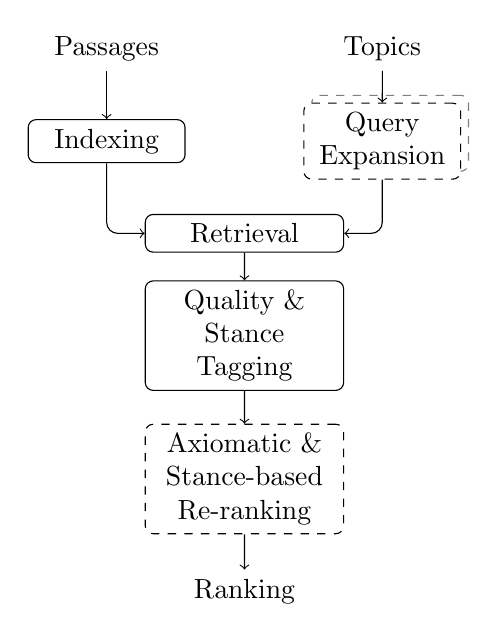
\begin{tikzpicture}[
        xscale=3.5,
        yscale=-1.3,
        block/.style={
            rectangle,
            draw,
            fill=white,
            text centered,
            rounded corners=1mm,
            text width=6.5em,
            minimum height=1em
        },
        line/.style={
            draw,
            ->,
            rounded corners
        },
      ]
        \node (documents) at (0,0) {Passages};
        \node (topics) at (1,0) {Topics};
        \node [block,text width=5em] (index) at (0,0.9) {Indexing};
        \node [block,dashed,draw opacity=0.5,xshift=1mm,yshift=1mm,text width=5em] at (1,0.9) {Query\\Expansion};
        \node [block,dashed,text width=5em] (query-expansion) at (1,0.9) {Query\\Expansion};
        \node [block] (retrieval) at (0.5,1.8) {Retrieval};
        \node [block] (quality-stance-tagging) at (0.5,2.8) {Quality~\& Stance Tagging};
        \node [block,dashed] (reranking) at (0.5,4.2) {Axiomatic~\& Stance-based Re-ranking};
        \node (ranking) at (0.5,5.3) {Ranking};
        \path [line] (documents) -- (index);
        \path [line] (topics) -- (query-expansion);
        \path [line] (index) |- (retrieval);
        \path [line] (query-expansion) |- (retrieval);
        \path [line] (retrieval) -- (quality-stance-tagging);
        \path [line] (quality-stance-tagging) -- (reranking);
        \path [line] (reranking) -- (ranking);
      \end{tikzpicture}
    \end{figure}  
  \end{minipage}
\end{frame}

\begin{frame}{Submitted Runs}
  \begin{enumerate}
    \setlength{\itemsep}{2.5ex}
    \item Query Likelihood Baseline \\
    {\footnotesize Dirichlet smoothing, stance from IBM Debater (threshold~0.125)}
    \item Argument Axioms \\
    {\footnotesize \textsc{KwikSort} re-ranking with 7~argumentative IR axioms}
    \item Stance-based Re-ranking with Argument Axioms \\
    {\footnotesize balance stance exposure (pro~A vs. pro~B)}
    \item All You Need is T0 \\
    {\footnotesize expand \& generate queries, estimate argument quality \& stance \\ by prompting T0++}
    \item Argumentative Stance-based Re-ranking with T0 \\
    {\footnotesize expand \& generate queries with T0++ and fastText, stance from IBM Debater, axiomatic and stance-based re-ranking}
  \end{enumerate}
\end{frame}

\begin{frame}{Results \& Conclusion}
  \begin{block}{Retrieval}
    \begin{itemize}
      \item Dirichlet baseline worse than BM25 baseline~\cite{BondarenkoFKSGBPBSWPH2022}
      \item T0++ query expansion decreases nDCG@5
      \item stance-based re-ranking (balancing) can slightly increase nDCG@5
      \item re-ranking can't compensate the bad Dirichlet retrieval performance
    \end{itemize}
  \end{block}
  \begin{block}{Stance detection}
    \begin{itemize}
      \item T0++ stance prediction achieves highest macro-averaged F$_1$-score
      \item different number of ground-truth labels per team limits comparability
      \item with only top-5 (i.e., all approaches have ground-truth labels up to that depth): T0++ falls behind Team Levi's approaches
      \item unclear how to account for sampling bias
    \end{itemize}
  \end{block}
\end{frame}

\begin{frame}{Conclusion}
  \begin{itemize}
    \setlength{\itemsep}{2ex}
    \item[\faIcon{github}] \href{https://github.com/heinrichreimer/grimjack}{\texttt{heinrichreimer/grimjack}}
    \item T0 approaches rather unsuccessful
    \item balancing pro A and pro B arguments helps
    \item can't distinguish neutral from no stance
    \item unclear evaluation wrt. stance classification
  \end{itemize}
  \vspace{2ex}
  \begin{block}{Future Work}
    \begin{itemize}
      \setlength{\itemsep}{2ex}
      \item Dirichlet vs. BM25
      \item reproduce \& evaluate stance prediction on independent test dataset
    \end{itemize}
  \end{block}
  \only<1>{\color{white}}\only<2->{}%
  \begin{flushright}
    \thankyou \\
    {\itshape\scriptsize Thanks to the Friends of SIGIR for waiving my registration fee.}
  \end{flushright}
\end{frame}

\appendix
\section{\appendixname}

\bibliographyframe

\begin{frame}{Axiomatic Re-ranking with \texttt{\large ir\_axioms}~\cite{BondarenkoFRSVH2022}}
  \begin{itemize}
    \item \textsc{KwikSort}: re-rank based on pairwise axiomatic preferences
    \item majority vote: only if \(\geq 50\,\%\) axioms agree, change ranking
  \end{itemize}
  \begin{table}
    \renewcommand{\tabcolsep}{0.2em}
    \begin{tabularx}{\linewidth}{@{}lX@{}}
      \toprule
      \textbf{Name} & \textbf{Description} \\
      \midrule
      ArgUC~\cite{BondarenkoHVSPB2018} & Prefer more argumentative units. \\
      QTArg~\cite{BondarenkoHVSPB2018} & Prefer more query terms in argumentative units. \\
      QTPArg~\cite{BondarenkoHVSPB2018} & Prefer earlier query terms in argumentative units. \\
      CompArg & Prefer more comparative objects in argumentative units. \\
      CompPArg& Prefer earlier comparative objects in argumentative units. \\
      aSLDoc~\cite{BondarenkoFKHVS2019} & Prefer passages with 12--20 words per s15-18entence. \\
      ArgQ & Prefer higher argument quality. \\ 
      \bottomrule
    \end{tabularx}
  \end{table}
\end{frame}

\begin{frame}{Query Reformulation with T0++~\cite{SanhWRBSACSLRDBXTSSKCNDCJWMSYPBWNRSSFFTBGBWR2021}}
  \begin{itemize}
    \item prompt: \texttt{\fontsize{7.2pt}{7.2pt}\selectfont <text>.\ Extract a natural search query from this description.}
    \item with \texttt{\fontsize{7.2pt}{7.2pt}\selectfont <text>} being the topic description~(D) or narrative~(N)
  \end{itemize}
  \begin{table}
    \renewcommand{\tabcolsep}{0.2em}
    \footnotesize
    \begin{tabularx}{\linewidth}{>{\hsize=.7\hsize\linewidth=\hsize}X c >{\hsize=1.3\hsize\linewidth=\hsize}X}
      \toprule
      \textbf{Topic} & \textbf{Field} & \textbf{Generated query} \\
      \midrule
      \multirow{2}{\linewidth}{Train or plane? Which is the better choice?} & D & Travel \\
      & N & What are the benefits of trains over planes for intercontinental travel? \\
      \multirow{2}{\linewidth}{Should I major in philosophy or psychology?} & D & What is the difference between philosophy and psychology? \\
      & N & What are the benefits of a major in English or history? \\
      \bottomrule
    \end{tabularx}
  \end{table}
\end{frame}

\end{document}